%%%%%%%%%%%%%%%%%%%%%%%%%%%%%%%%%%%%%%%%%
% Beamer Presentation
% LaTeX Template
% Version 1.0 (10/11/12)
%
% This template has been downloaded from:
% http://www.LaTeXTemplates.com
%
% License:
% CC BY-NC-SA 3.0 (http://creativecommons.org/licenses/by-nc-sa/3.0/)
%
%%%%%%%%%%%%%%%%%%%%%%%%%%%%%%%%%%%%%%%%%

%----------------------------------------------------------------------------------------
%	PACKAGES AND THEMES
%----------------------------------------------------------------------------------------

\documentclass[UTF8,aspectratio=169,14pt]{ctexbeamer}

\usepackage{hyperref}
\hypersetup{
	colorlinks=true,
	linkcolor=red,
	anchorcolor=blue,
	citecolor=green
}

\mode<presentation> {
	
	% The Beamer class comes with a number of default slide themes
	% which change the colors and layouts of slides. Below this is a list
	% of all the themes, uncomment each in turn to see what they look like.
	
	%\usetheme{default}
	%\usetheme{AnnArbor}
	%\usetheme{Antibes}
	%\usetheme{Bergen}
	%\usetheme{Berkeley}
	%\usetheme{Berlin}
	%\usetheme{Boadilla}
	%\usetheme{CambridgeUS}
	%\usetheme{Copenhagen}
	%\usetheme{Darmstadt}
	%\usetheme{Dresden}
	%\usetheme{Frankfurt}
	%\usetheme{Goettingen}
	%\usetheme{Hannover}
	%\usetheme{Ilmenau}
	%\usetheme{JuanLesPins}
	%\usetheme{Luebeck}
	\usetheme{Madrid}
	%\usetheme{Malmoe}
	%\usetheme{Marburg}
	%\usetheme{Montpellier}
	%\usetheme{PaloAlto}
	%\usetheme{Pittsburgh}
	%\usetheme{Rochester}
	%\usetheme{Singapore}
	%\usetheme{Szeged}
	%\usetheme{Warsaw}
	
	% As well as themes, the Beamer class has a number of color themes
	% for any slide theme. Uncomment each of these in turn to see how it
	% changes the colors of your current slide theme.
	
	%\usecolortheme{albatross}
	%\usecolortheme{beaver}
	%\usecolortheme{beetle}
	%\usecolortheme{crane}
	%\usecolortheme{dolphin}
	%\usecolortheme{dove}
	%\usecolortheme{fly}
	%\usecolortheme{lily}
	%\usecolortheme{orchid}
	%\usecolortheme{rose}
	%\usecolortheme{seagull}
	%\usecolortheme{seahorse}
	%\usecolortheme{whale}
	%\usecolortheme{wolverine}
	
	%\setbeamertemplate{footline} % To remove the footer line in all slides uncomment this line
	%\setbeamertemplate{footline}[page number] % To replace the footer line in all slides with a simple slide count uncomment this line
	
	%\setbeamertemplate{navigation symbols}{} % To remove the navigation symbols from the bottom of all slides uncomment this line
}

\usepackage{graphicx} % Allows including images
\graphicspath{{./figs/}}
\usepackage{booktabs} % Allows the use of \toprule, \midrule and \bottomrule in tables
\usepackage{longtable}
\usepackage{listings}
\usepackage{xcolor}
\lstset{numbers=left, %设置行号位置
	numberstyle=\tiny, %设置行号大小
	keywordstyle=\color{blue}, %设置关键字颜色
	commentstyle=\color[cmyk]{1,0,1,0}, %设置注释颜色
	frame=single, %设置边框格式
	escapeinside=``, %逃逸字符(1左面的键),用于显示中文
	%breaklines, %自动折行
	extendedchars=false, %解决代码跨页时,章节标题,页眉等汉字不显示的问题
	xleftmargin=2em,xrightmargin=2em, aboveskip=1em, %设置边距
	tabsize=4, %设置tab空格数
	showspaces=false %不显示空格
}
% Fonts
% \usepackage{libertine}
% \setmonofont{Courier}
\setCJKsansfont[ItalicFont=Noto Serif CJK SC Black, BoldFont=Noto Sans CJK SC Black]{Noto Sans CJK SC}


%----------------------------------------------------------------------------------------
% TITLE PAGE
%----------------------------------------------------------------------------------------

\title[第21讲]{第二十一讲 :异步编程(Asynchronous Programming)} % The short title appears at the bottom of every slide, the full title is only on the title page
\subtitle{第1节:Background}
\author{向勇、陈渝} % Your name
\institute[清华大学] % Your institution as it will appear on the bottom of every slide, may be shorthand to save space
{
  清华大学计算机系 \\ % Your institution for the title page
  \medskip
  \textit{xyong,yuchen@tsinghua.edu.cn} % Your email address
}
\date{\today} % Date, can be changed to a custom date

\begin{document}

\begin{frame}
\titlepage % Print the title page as the first slide
\end{frame}

%----------------------------------------------
\begin{frame}
\frametitle{提纲} % Table of contents slide, comment this block out to remove it
\tableofcontents % Throughout your presentation, if you choose to use \section{} and \subsection{} commands, these will automatically be printed on this slide as an overview of your presentation
% itemize
Ref:
    \begin{itemize}
        \item \href{https://cfsamson.github.io/books-futures-explained/}{Futures Explained in 200 Lines of Rust}
        \item Writing an OS in Rust - \href{https://os.phil-opp.com/async-await/}{Async/Await}
        \item \href{https://zhuanlan.zhihu.com/p/97574385}{零成本异步I/O}
    \end{itemize}

\end{frame}
%----------------------------------------------
% ### ref
% 
% - [Futures Explained in 200 Lines of Rust](https://cfsamson.github.io/books-futures-explained/#futures-explained-in-200-lines-of-rust) [repo at github](https://github.com/cfsamson/books-futures-explained)
% - Writing an OS in Rust - [Async/Await](https://os.phil-opp.com/async-await/)
% - [零成本异步I/O](https://zhuanlan.zhihu.com/p/97574385)
% 
%----------------------------------------------
%%  PRESENTATION SLIDES
%----------------------------------------------
\section{Background} % Sections can be created in order to organize your presentation into discrete blocks, all sections and subsections are automatically printed in the table of contents as an overview of the talk
\section{Futures in Rust} % Sections can be created in order to organize your presentation into discrete blocks, all sections and subsections are automatically printed in the table of contents as an overview of the talk
\section{Generators and async/await} % Sections can be created in order to organize your presentation into discrete blocks, all sections and subsections are automatically printed in the table of contents as an overview of the talk
\section{Self-Referential Structs \& Pin} % Sections can be created in order to organize your presentation into discrete blocks, all sections and subsections are automatically printed in the table of contents as an overview of the talk
\section{Waker and Reactor} % Sections can be created in order to organize your presentation into discrete blocks, all sections and subsections are automatically printed in the table of contents as an overview of the talk
%----------------------------------------------
%\subsection{xxxx} % A subsection can be created just before a set of slides with a common theme to further break down your presentation into chunks
%----------------------------------------------
\begin{frame}[fragile]
    \frametitle{Multitasking}
%    \framesubtitle{xxxx}
% ### 21.1 Background
% ref: https://cfsamson.github.io/books-futures-explained/0_background_information.html#some-background-information
% 
% 
% #### Multitasking
% 
% 参考: https://cfsamson.github.io/book-exploring-async-basics/2_async_history.html#non-preemptive-multitasking
% 
{\color{red}Non-Preemptive multitasking}
 %% itemize
     \begin{itemize}
         \item The programmer `yielded` control to the OS
         \item Every bug could halt the entire system
         \item Example: Windows 95
     \end{itemize}
 
{\color{red}Preemptive multitasking}
 %% itemize
     \begin{itemize}
         \item OS can stop the execution of a process, do something else, and switch back
         \item OS is responsible for scheduling tasks
         \item Example: UNIX, Linux
     \end{itemize}
% 
\end{frame}
%----------------------------------------------
\begin{frame}[fragile]
    \frametitle{User-level Thread}
%    \framesubtitle{xxxx}
% #### User-level Thread
% 
% 参考: https://stackoverflow.com/questions/15983872/difference-between-user-level-and-kernel-supported-threads
% 
% https://cfsamson.github.io/books-futures-explained/0_background_information.html#green-threads
% 
{\color{red}Advantages}
 
 %% itemize
     \begin{itemize}
         \item Simple to use
         \item A "context switch" is reasonably fast
         \item Each stack only gets a little memory
     	\begin{itemize}
     	    \item You can have hundreds of thousands of user-level threads running
       \end{itemize}
         \item Easy to incorporate preemption
     \end{itemize}
 
{\color{red}Drawbacks}
 
%% itemize
    \begin{itemize}
        \item The stacks might need to grow
    	\begin{itemize}
    	    \item Solving this is not easy and will have a cost
      \end{itemize}
        \item Need to save all the CPU state on every switch
        \item Complicated to implement correctly if you want to support many different platforms
    \end{itemize}

Example: \href{https://cfsamson.github.io/books-futures-explained/0_background_information.html#green-threads}{Green Threads}

\end{frame}
%----------------------------------------------
\begin{frame}[fragile]
    \frametitle{Kernel-supported Threads}
%    \framesubtitle{xxxx}
% #### Kernel-supported Threads
% 
% ref: https://stackoverflow.com/questions/15983872/difference-between-user-level-and-kernel-supported-threads
% https://cfsamson.github.io/books-futures-explained/0_background_information.html#threads-provided-by-the-operating-system
% 
{\color{red}Advantages}
 
 %% itemize
     \begin{itemize}
         \item Easy to use
         \item Switching between tasks is reasonably fast
         \item Geting parallelism for free
     \end{itemize}
 
{\color{red}Drawbacks}
 
 %% itemize
     \begin{itemize}
         \item OS level threads come with a rather large stack
         \item There are a lot of syscalls involved
         \item Might not be an option on some systems, such as http server
     \end{itemize}
 
 Example:
 
 %% itemize
     \begin{itemize}
         \item \href{https://cfsamson.github.io/books-futures-explained/0_background_information.html#threads-provided-by-the-operating-system}{Using OS threads in Rust}
     \end{itemize}
 
\end{frame}
%----------------------------------------------
\begin{frame}[fragile]
    \frametitle{Callback based approaches}
%    \framesubtitle{xxxx}
% #### Callback based approaches
% 
% Ref: https://cfsamson.github.io/books-futures-explained/0_background_information.html#callback-based-approaches
% 
 A callback based approach is to save a pointer to a set of instructions we want to run later together with whatever state is needed.
 
{\color{red}Advantages}
 
 %% itemize
     \begin{itemize}
         \item Easy to implement in most languages
         \item No context switching
         \item Relatively low memory overhead
     \end{itemize}
 
{\color{red}Drawbacks}
 
 %% itemize
     \begin{itemize}
         \item Memory usage grows linearly with the number of callbacks
     	\begin{itemize}
     	    \item Each task must save the state it needs for later
     	\end{itemize}
         \item Callback hell: Hard to debug
         \item Require a substantial rewrite to go from a "normal" program flow to one that uses a "callback based" flow
     \end{itemize}
 
Example: \href{https://cfsamson.github.io/books-futures-explained/0_background_information.html#callback-based-approaches}{Callback based approaches}
 
\end{frame}
%----------------------------------------------
\begin{frame}[fragile]
    \frametitle{Event queue: Epoll, Kqueue and IOCP}
%    \framesubtitle{xxxx}
% #### Event queue: Epoll, Kqueue and IOCP
% 
% 参考: https://cfsamson.github.io/book-exploring-async-basics/6_epoll_kqueue_iocp.html#epoll
% https://zhuanlan.zhihu.com/p/39970630 select poll epoll的区别
% 
% There are some well-known libraries which implement a cross platform event queue using Epoll, Kqueue and IOCP for Linux, Mac, and Windows, respectively.
% 
%% itemize
    \begin{itemize}
        \item Epoll
    	\begin{itemize}
    	    \item Epoll is the Linux way of implementing an event queue
    	    \item Epoll was designed to work very efficiently with a large number of events
    	\end{itemize}
        \item Kqueue
    	\begin{itemize}
    	    \item Kqueue is the MacOS way of implementing an event queue, which originated from BSD
    	    \item In terms of high level functionality, it's similar to Epoll in concept but different in actual use
    	\end{itemize}
        \item IOCP
    	\begin{itemize}
    	    \item IOCP or Input Output Completion Ports is the way Windows handles this type of event queue
    	\end{itemize}
    \end{itemize}

\end{frame}
%----------------------------------------------
\begin{frame}[fragile]
    \frametitle{Epoll}
%    \framesubtitle{xxxx}
% #### Epoll
% 
% 参考: https://zhuanlan.zhihu.com/p/39970630
% 
%% figure
    \begin{figure}
    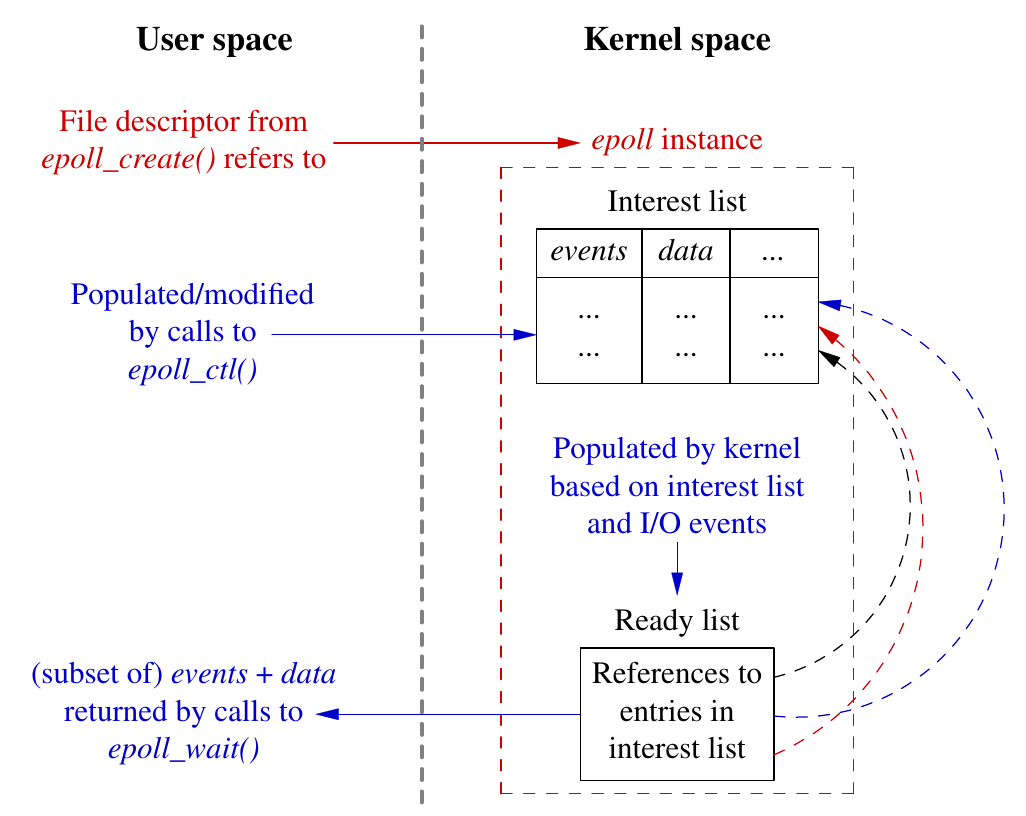
\includegraphics[width=0.55\linewidth]{figs/epoll.png}
%    \caption{xxxx}
    \end{figure}
% ![epoll](figs/epoll.png)
% 
\end{frame}
%----------------------------------------------
\begin{frame}[fragile]
    \frametitle{Procedure for read data from a socket using epoll}
%    \framesubtitle{xxxx}
% #### Read data from a socket using epoll
% 
% https://cfsamson.github.io/book-exploring-async-basics/6_epoll_kqueue_iocp.html#readiness-based-event-queues
% 
% {\color{red}Workflow to read data from a socket using epoll/kqueue}
% 
    \begin{enumerate}
        \item Create an event queue by calling the syscall `epoll\_create` or `kqueue`
        \item Ask the OS for a file descriptor representing a network socket
        \item Register an interest in `Read` events on this socket
    	\begin{itemize}
    	    \item In order to receive a notification when the event is ready in the event queue we created
    	\end{itemize}
        \item Call `epoll\_wait` or `kevent` to wait for an event
    	\begin{itemize}
    	    \item Block (suspend) the thread it's called on
    	\end{itemize}
        \item When the event is ready, our thread is resumed, and return from our "wait" call with data about the event
        \item Call `read` on the socket we created
    \end{enumerate}
% 
{\color{red}Example}
% 
%% itemize
    \begin{itemize}
        \item \href{http://man7.org/linux/man-pages/man7/epoll.7.html}{Epoll example}
        \item \href{https://www.suchprogramming.com/epoll-in-3-easy-steps/}{Complete example}
    \end{itemize}

\end{frame}
%----------------------------------------------
\begin{frame}[fragile]
    \frametitle{From callbacks to futures (deferred computation)}
%    \framesubtitle{xxxx}
% #### From callbacks to futures (deferred computation)
% 
% ref: https://cfsamson.github.io/books-futures-explained/0_background_information.html#from-callbacks-to-promises
% 
Future is one way to deal with the complexity which comes with a callback based approach.
\begin{block}{}
\begin{verbatim}
//rust code
async function run() {
    await timer(200);
    await timer(100);
    await timer(50);
    console.log("I'm the last one");
}
\end{verbatim}
\end{block}
% 
% 
%% itemize
    \begin{itemize}
        \item The `run` function as a *pausable* task consisting of several sub-tasks
    	\begin{itemize}
    	    \item On each "await" point it yields control to the scheduler
    	\end{itemize}
        \item When the sub-tasks changes state to either `fulfilled` or `rejected`, the task is scheduled to continue to the next step
    \end{itemize}

\end{frame}
%----------------------------------------------
\end{document}
